\documentclass[a4paper, 12pt]{book}
% preamble.tex

\usepackage[utf8]{inputenc}
\usepackage[T1]{fontenc}
\usepackage[english]{babel} % Ho cambiato in italian, supponendo che la maggior parte del testo sia in italiano
\usepackage{amsmath}
\usepackage{amssymb}
\usepackage{graphicx}
\usepackage{hyperref}
\usepackage{geometry}
\usepackage{fontspec} % Utile per Xetex/LuaLaTeX ma mantenuto
\usepackage{booktabs}
\usepackage{amsthm}
\usepackage{enumitem}
\usepackage{caption}
\usepackage{thmtools}
\usepackage{standalone} % Già presente nel tuo elenco
\usepackage{tkz-euclide}
\usepackage{graphicx}
\usepackage[T1]{fontenc}
\usepackage{wesa}

% --- PACCHETTI AGGIUNTI PER LA FORMATTAZIONE ---
\usepackage{parskip}  % Aggiunge spazio tra i paragrafi (stile "blocco")
\usepackage{fancyhdr} % Per intestazioni e piè di pagina personalizzati

% --- IMPOSTAZIONI GEOMETRIA E FONT ---
\geometry{a4paper, margin=1in}

% Configura lo stile 'plain' (usato da \maketitle e \tableofcontents)
% per essere coerente con il piè di pagina
\fancypagestyle{plain}{
    \fancyhf{} % Pulisce
    \cfoot{\thepage} % Mette solo il numero di pagina
    \renewcommand{\headrulewidth}{0pt} % Niente linea su queste pagine
}

% Configurazione Header/Footer per le altre pagine
\pagestyle{fancy}
\fancyhead{} % Pulisce l'intestazione
\fancyfoot{} % Pulisce il piè di pagina
\fancyhead[L]{\nouppercase{\rightmark}} % Nome Sezione a sinistra (o Chapter)
\fancyhead[R]{\nouppercase{\leftmark}}  % Nome Capitolo a destra (o Sezione)
\fancyfoot[C]{\thepage} % Numero di pagina al centro
\renewcommand{\headrulewidth}{0.4pt}
\renewcommand{\footrulewidth}{0pt}


% --- DEFINIZIONI TEOREMI ---
% (Questa parte è cruciale per la tua struttura)
\newtheoremstyle{mythmstyle}%
    {}%
    {}%
    {\itshape}%
    {}%
    {\bfseries}%
    {}%
    { }%
    {\thmname{#1}\thmnumber{ #2}%
    \thmnote{: #3\addcontentsline{toc}{subsubsection}{{\itshape#1}: #3}}. }

% 2. Imposta questo stile come quello ATTUALE
\theoremstyle{mythmstyle}

\newtheorem{theorem}{Th}[section]
\newtheorem{definition}{Def}[section]
\newtheorem{proposition}{Prop}[section]
\newtheorem{corollary}{Cor}[section]
\newtheorem{algorithm}{Alg}[section]
\newtheorem{lemma}{Lemma}[section]
\newtheorem*{remark}{Rem}

% Definizioni utili per il Main file
\newcommand{\inputlesson}[1]{\clearpage\input{#1}\clearpage} % Comando per input lezione

\usepackage{tikz}
\usetikzlibrary{shapes,fit}
\usepackage{pgfplots}
\pgfplotsset{compat=1.18}
\usepackage{amsmath} % Required for align environment
\usepackage{caption} % Required for \captionof outside float environments



\begin{document}
\setcounter{chapter}{12}
\chapter{Lesson 12-12-2025}
\section{Frequency selectivity}
\hfill 12/12/2025

\subsection{Important parameters ($R_h, T_d$, PDP) and WSSUS assumption \{3.4.2\}}

% Flowchart Diagram Reconstruction
\begin{center}
\begin{tikzpicture}[
    node distance=1cm and 1cm,
    box/.style={
        rectangle, 
        draw=obsidianBorderPurple, 
        fill=obsidianPurple, 
        rounded corners, 
        align=center, 
        font=\footnotesize\sffamily,
        minimum height=1.5cm,
        inner sep=5pt
    },
    yellowbox/.style={
        rectangle,
        draw=yellow!80!orange,
        fill=obsidianYellow,
        align=center,
        font=\footnotesize\sffamily
    },
    arrow/.style={-Latex, draw=black!70}
]

    % Nodes
    \node[yellowbox] (now) {Now};
    \node[box, below=0.1cm of now] (flatness) {Frequency flatness,\\ frequency correlation\\ and coherence\\ bandwidth};
    
    \node[box, right=of flatness] (relation) {Relation between\\ period, delays and\\ frequency-\\ flatness/selectivity};
    
    \node[box, right=of relation] (pdp) {Power delay profile\\ and its relation with\\ the frequency\\ correlation};
    
    \node[box, below right=0.5cm and -0.5cm of pdp] (delay) {Delay spread in\\ continuous and\\ discrete cases};
    
    \node[box, above right=0.5cm and -0.5cm of pdp] (wssus) {WSSUS assumption};

    % Arrows
    \draw[arrow] (flatness) -- (relation);
    \draw[arrow] (relation) -- (pdp);
    \draw[arrow] (pdp) -- (wssus);
    \draw[arrow] (pdp) -- (delay);
    \draw[arrow] (wssus) to[bend left=20] (pdp); % Small return arrow implied by context
    
\end{tikzpicture}
\end{center}

Now we'll talk about the coherence bandwidth $B_c$; in order to do so, we define $R_h$ which looks kinda like a correlation.

\begin{yellowbox}[\faBook\ \textit{Channel modeling} (pp. 131-208), p. 28]
In our characterization of space and time selectivity, we have focused on the fading experienced by a sinusoid (both for what concerns the influence of {\color{green!60!black} space correlation} and, although implicitly, the influence of {\color{green!60!black} time correlation}) at frequency $f_c$. The derivations hold approximately for frequencies close enough to $f_c$, and thus the fading goes (roughly) unchanged over a certain frequency span. \textbf{If the entire signal fits within a swath of frequencies that experience (roughly) the same fading, the fading is frequency-flat}; the channel is then multiplicative, i.e., it merely applies a complex gain. The signal can also be said to be narrowband, although such narrowness must be understood only in reference to the fading.
\end{yellowbox}

\begin{yellowbox}[\faBook\ \textit{Channel modeling} (pp. 131-208), p. 28]
If the signal bandwidth is large enough, however, it is bound to exceed the range of frequencies experiencing (roughly) the same fading. At a given location then, in static conditions, the noiseless received signal is $y(f) = \sqrt{G} h(f) x(f)$ where $h(f)$ is no longer constant over the bandwidth $B$. \textbf{The signal undergoes frequency-selective fading}, and it can be said to be fading-wise wideband; the channel is not merely multiplicative, but rather it effects a nontrivial convolution that modifies the shape of the symbol pulses. The degree of selectivity over a frequency range $\Delta_f$ is quantified by
\begin{align}
    R_h(\Delta_f) = \mathbb{E}[h(f)h^*(f+\Delta_f)]
\end{align}
\textit{\color{red} \faPen\ Note: what is implied in this formula? There is a dependency only in $\Delta f$, but it should be on $f$ and $\Delta f$ (depends only on $\Delta f$).}

whose chief measure is the \textbf{coherence bandwidth} $B_c$, the natural counterpart to the coherence time and the coherence distance. \textbf{The fading is frequency-flat if $B \ll B_c$}.
\end{yellowbox}

\begin{purplebox}[\faPen\ Handwritten Note]
For most channels this is true in general,
$e^{j2\pi f_0 t^2} \xrightarrow{\text{der}} \frac{1}{2\pi}\frac{d}{dt}(2\pi f_0 t^2) \implies f_0 t \to$ \tikz[baseline=-0.5ex]{\draw (0,0) -- (0.5,0.5) node[right] {$f$};}
\end{purplebox}

We ask ourselves the question: if we take a frequency and another frequency separated of $\Delta_f$ from the first one, which is the difference in terms of the channel?
We can see that \textbf{the function $R_h$ does not depend on the frequency} (in fact, it's expressed as $R_h(\Delta_f)$ and not as $R_h(\Delta_f, f)$); \begin{yellowbox} this is not always true: it's like when we show that the correlation of the stationary process only depends on the difference over time.\end{yellowbox}

Depending on what the shape of $h(f)$ is, we can define what the coherence bandwidth is.

\begin{bluebox}[\faPen\ Possible definition of Coherence Bandwidth $B_c$]
The coherence bandwidth is sloppy as a concept; just to give an example of definition:

\begin{center}
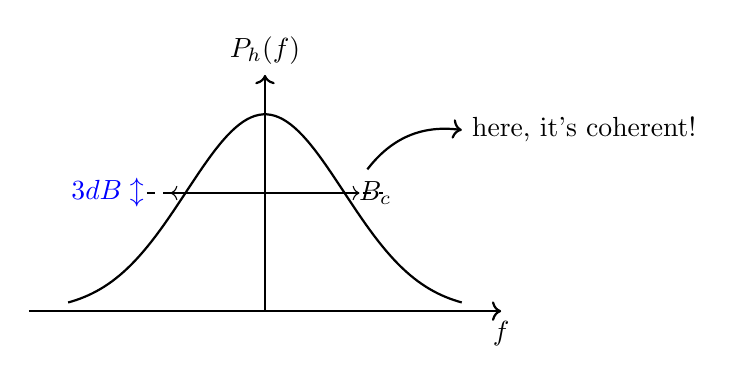
\begin{tikzpicture}
    % Axis
    \draw[->, thick] (-3,0) -- (3,0) node[below] {$f$};
    \draw[->, thick] (0,0) -- (0,3) node[above] {$P_h(f)$};
    
    % Gaussian curve
    \draw[thick] plot [domain=-2.5:2.5, samples=100] (\x, {2.5*exp(-\x*\x/2)});
    
    % 3dB line
    \draw[dashed] (-1.5, 1.5) -- (1.5, 1.5);
    \node[blue] at (-2, 1.5) {$3dB \updownarrow$};
    
    % Bc arrows
    \draw[<->] (-1.2, 1.5) -- (1.2, 1.5);
    \node at (1.4, 1.5) {$B_c$};
    
    % Coherent note
    \draw[->, thick, bend left] (1.3, 1.8) to (2.5, 2.3) node[right] {here, it's coherent!};
\end{tikzpicture}
\end{center}

we might decide it's 3dB from the top.
\end{bluebox}

The \textbf{coherence bandwidth} is that bandwidth in which the channel stays almost constant; this is extremely important when we do OFDM, since that tells us where we can position a pilot without having a frequency-dependent distortion.

\begin{figure}[h]
    \centering
    
\includegraphics[width=0.6\textwidth]{Pictures/image.png}
    \caption{Coherence bandwidth}
    \label{fig:coherence_bandwidth}
\end{figure}

We can put the pilots spaced of not more than the coherence bandwidth; if we do more, the channel in the middle can change.
This is definitely important; citing the slides: "Coherence bandwidth $B_c$ determines the bandwidths where the channel should be considered frequency selective".

This means that somehow in the previous example we have 2 different channels which are {\color{green!60!black} frequency selective}:

\begin{figure}[h]
    \centering
    
\includegraphics[width=0.6\textwidth]{Pictures/image copy.png}
\end{figure}

Normally, the \textbf{time-invariant impulse response corresponding to $h(f)$ is $h(\tau) = h\delta(\tau)$, with $h$ being a complex gain at a given position}. Of course, if we were to introduce motion, it'd become time-dependent, giving $h(t, \tau) = h(t)\delta(\tau)$.

% Repeat Flowchart (Simplified as visual cue)
\begin{center}
\begin{tikzpicture}[scale=0.8, transform shape,
    node distance=0.8cm and 0.8cm,
    box/.style={rectangle, draw=obsidianBorderPurple, fill=obsidianPurple, rounded corners, align=center, font=\tiny\sffamily, inner sep=3pt},
    yellowbox/.style={rectangle, draw=yellow!80!orange, fill=obsidianYellow, align=center, font=\tiny\sffamily},
    arrow/.style={-Latex, draw=black!70}
]
    \node[yellowbox] (now) {Now};
    \node[box, below=0.1cm of now] (flatness) {Frequency flatness,\\ frequency correlation\\ and coherence\\ bandwidth};
    \node[box, right=of flatness] (relation) {Relation between\\ period, delays and\\ frequency-\\ flatness/selectivity};
    \node[box, right=of relation] (pdp) {Power delay profile\\ and its relation with\\ the frequency\\ correlation};
    \node[box, below right=0.3cm and -0.3cm of pdp] (delay) {Delay spread in\\ continuous and\\ discrete cases};
    \node[box, above right=0.3cm and -0.3cm of pdp] (wssus) {WSSUS assumption};

    \draw[arrow] (flatness) -- (relation);
    \draw[arrow] (relation) -- (pdp);
    \draw[arrow] (pdp) -- (wssus);
    \draw[arrow] (pdp) -- (delay);
\end{tikzpicture}
\end{center}

If we consider a \textbf{motionless channel} for which the minimum and maximum delays are $\tau_{\min}, \tau_{\max}$, we'd then have that if $\tau_{\max} - \tau_{\min} \ll T$ (with $T$ being the symbol period), then we'd have that the channel can still be modeled as $h(\tau) = h\delta(\tau)$ with little error.
If instead the condition is not satisfied, there is collision between the symbol $n$ from a certain path and the symbols $\neq n$ from other paths, causing not only fading but also ISI.

\begin{yellowbox}[\faBook\ \textit{Channel modeling} (pp. 131-208), p. 29]
To be sure, any form of fading is the result of self-interference among multipath signal replicas of each symbol; the difference between frequency-flat and frequency-selective fading is that, in the former, every symbol essentially interferes exclusively with replicas of itself, whereas \textbf{in the latter it experiences significant interference with adjacent symbols as well}. The same exact channel \textbf{can exhibit either frequency-flat or frequency-selective fading depending on $T$ or, equivalently, depending on the bandwidth through which it is observed.}
\end{yellowbox}

\begin{yellowbox}[\faBook\ \textit{Channel modeling} (pp. 131-208), p. 29]
Ultimately, the delay-dispersive nature of fading channels, and thus the frequency selectivity, is rooted in the fact that the speed of light is finite. To appreciate this, the reader is referred to Fig. 3.14, which depicts a transmit sequence of symbols traveling over two distinct propagation paths. The finite value of $c$ bestows upon the symbol separation a finite length in space and opens the door to distinct symbols colliding at the receiver if the difference in length between the paths is sufficiently large. In contrast, if $c$ were infinite, then the symbol sequences received over the multiple paths would always align.
The foregoing interpretation can be further stretched to motivate the use of OFDM: since ISI arises because of the finite length of the symbols, \textbf{the antidote to ISI is to make the symbols longer}.
\end{yellowbox}

\begin{figure}[h]
    \centering
    
\includegraphics[width=0.7\textwidth]{Pictures/immagine-000.png}
\end{figure}

Symbol sequence traveling over two distinct propagation paths with lengths differing by substantially more than the symbol period. The sequences received over the two paths are staggered by about half a period, which for $T = 3.7\ \mu\text{s}$ would happen if the path lengths differed by about 500 m.

% Flowchart Highlight: Power Delay Profile
\begin{center}
\begin{tikzpicture}[
    node distance=1cm and 1cm,
    box/.style={
        rectangle, 
        draw=obsidianBorderPurple, 
        fill=obsidianPurple, 
        rounded corners, 
        align=center, 
        font=\footnotesize\sffamily,
        minimum height=1.5cm,
        inner sep=5pt
    },
    activebox/.style={
        rectangle, 
        draw=obsidianBorderPurple, 
        fill=obsidianPurple!40!gray, % Slightly darker to indicate active but keeping style
        rounded corners, 
        align=center, 
        font=\footnotesize\sffamily,
        minimum height=1.5cm,
        inner sep=5pt
    },
    yellowbox/.style={
        rectangle,
        draw=yellow!80!orange,
        fill=obsidianYellow,
        align=center,
        font=\footnotesize\sffamily
    },
    arrow/.style={-Latex, draw=black!70}
]

    % Nodes
    \node[yellowbox] (now) {Now};
    \node[box, below=0.1cm of now] (flatness) {Frequency flatness,\\ frequency correlation\\ and coherence\\ bandwidth};
    
    \node[box, right=of flatness] (relation) {Relation between\\ period, delays and\\ frequency-\\ flatness/selectivity};
    
    % This is the active one, wrapped in yellow box in source
    \node[yellowbox, right=of relation, minimum height=1.5cm, inner sep=5pt] (pdp) {Power delay profile\\ and its relation with\\ the frequency\\ correlation};
    
    \node[box, below right=0.5cm and -0.5cm of pdp] (delay) {Delay spread in\\ continuous and\\ discrete cases};
    
    \node[box, above right=0.5cm and -0.5cm of pdp] (wssus) {WSSUS assumption};

    % Arrows
    \draw[arrow] (flatness) -- (relation);
    \draw[arrow] (relation) -- (pdp);
    \draw[arrow] (pdp) -- (wssus);
    \draw[arrow] (pdp) -- (delay);
    \draw[arrow] (wssus) to[bend left=20] (pdp); 
    
\end{tikzpicture}
\end{center}

We can write down the \textbf{power delay profile (PDP)}, which \textbf{quantifies the energy distributed as a function of delay in the time domain}; it is normalized so that it can be interpreted as a PDF (describing how likely we are to have a certain amount of power at a certain delay) and it is denoted by
\begin{equation}
    S_h(\tau) = \mathbb{E}[|h(\tau)|^2]. \tag{3.68}
\end{equation}

\begin{yellowbox}[\faBook\ \textit{Channel modeling} (pp. 131-208), p. 31]
Although in general a continuous function of delay, discrete PDP descriptions are also possible, and in fact fairly common. In our formulation, these are readily accommodated by means of delay-shifted delta functions, each modeling a group of paths—a ray—with similar delays. Because of the plurality of paths per ray, each ray is still subject to fading.
\end{yellowbox}

For a certain $\tau$, we measure the expectation of the amplitude of the channel; if we have a \textbf{ray-based channel} (we have group of paths with similar delays), we'll get a \textbf{channel given by delayed deltas}:

\begin{figure}[h]
    \centering
    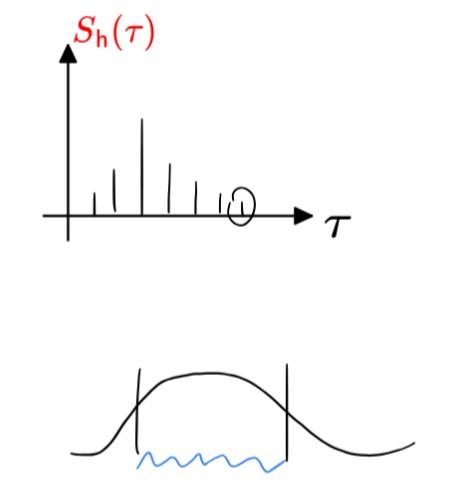
\includegraphics[width=0.5\textwidth]{Pictures/image copy 2.png}
\end{figure}

\begin{purplebox}[\faGhost\ What does that graph mean?]
I think the intuition is that a certain delay between two signals defines a certain bandwidth; if we know the average of the signal in that certain bandwidth, given by $S_h(\tau)$, we can draw some conclusions about the bandwidths at which we should transmit.
\end{purplebox}

This might allow us to put the various signals only in a certain part of the channel. The two quantities $R_h$ and $S_h$ are related through a transform.
First we have that
\begin{align}
    R_h(\Delta_f) &= \mathbb{E}[h(f)h^*(f+\Delta_f)] \tag{3.73} \\
    &= \mathbb{E} \left[ \left( \int_{-\infty}^{+\infty} h(\tau_0)e^{-j2\pi f \tau_0} \, d\tau_0 \right) \left( \int_{-\infty}^{+\infty} h^*(\tau_1)e^{j2\pi (f+\Delta_f) \tau_1} \, d\tau_1 \right) \right] \tag{3.74} \\
    &= \int_{-\infty}^{+\infty} \int_{-\infty}^{+\infty} \mathbb{E}[h(\tau_0)h^*(\tau_1)] e^{j2\pi [(f+\Delta_f)\tau_1 - f\tau_0]} \, d\tau_0 \, d\tau_1 \tag{3.75}
\end{align}
but if we now consider a peculiar case (which is the \textbf{WSSUS case}, see below), aka that for which
\[
\mathbb{E}[h(\tau_0)h^*(\tau_1)] = 0 \quad \text{if } \tau_0 \neq \tau_1,
\]
we can now consider the integral only for $\tau = \tau_0 = \tau_1$, seeing that it reduces to
\begin{align}
    R_h(\Delta_f) &= \int_{-\infty}^{+\infty} \mathbb{E}[|h(\tau)|^2] e^{j2\pi \tau \Delta_f} \, d\tau \tag{3.76} \\
    &= \int_{-\infty}^{+\infty} S_h(\tau) e^{j2\pi \tau \Delta_f} \, d\tau . \tag{3.77}
\end{align}

The two are related with one another (the correlation over frequency differences is the \textbf{IFT of the power delay profile})!


\begin{purplebox}[\faGhost\ Elaborating further...]
The idea is that there is a tight relation between how our signal is distributed across delays ($S_h$) and how it is distributed in frequency ($R_h$): (3.77) allows us to draw a relation between the two values, furthermore allowing us to understand whether \textit{certain frequency difference spans} experience highly correlating signals (implying that the signal is really redundant) or perhaps mostly uncorrelated signals (implying that if said delay is achieved, the received signals across delays will contain little to no information about each other).
If we then consider $S_h(\tau)$ as a PDF, expressing the relative amount of power which is given to a delay, we can interpret (3.77) as an average of $e^{j2\pi\tau\Delta_f}$ across $\tau$.
\end{purplebox}

\begin{bluebox}[\faPen\ Coherence bandwidth]
Thanks to the relation between $R_h(\cdot)$ and $S_h(\cdot)$, we can write that
\begin{equation}
    B_c \propto \frac{1}{T_d} : \tag{3.78}
\end{equation}
this is the closest thing we have to a definition for the coherence bandwidth!!
\end{bluebox}

\begin{center}
\begin{tikzpicture}[
    node distance=1cm and 1cm,
    box/.style={
        rectangle, 
        draw=obsidianBorderPurple, 
        fill=obsidianPurple, 
        rounded corners, 
        align=center, 
        font=\footnotesize\sffamily,
        minimum height=1.3cm,
        inner sep=3pt
    },
    yellowbox/.style={
        rectangle,
        draw=yellow!80!orange,
        fill=obsidianYellow,
        align=center,
        font=\footnotesize\sffamily
    },
    arrow/.style={-Latex, draw=black!70}
]
    % Reconstruction of the partial flowchart shown
    \node[yellowbox] (now) {Now};
    
    \node[box, below left=0.5cm and 0.5cm of now] (pdp) {Power delay profile\\ and its relation with\\ the frequency\\ correlation};
    
    \node[box, left=of pdp] (relation) {Relation between\\ period, delays and\\ frequency-\\ flatness/selectivity};
    
    \node[box, left=of relation] (flatness) {Frequency flatness,\\ frequency correlation\\ and coherence\\ bandwidth};
    
    \node[yellowbox, below right=0.3cm and -0.8cm of now] (wssus) {WSSUS assumption};
    
    \node[box, below right=0.5cm and -0.5cm of pdp] (delay) {Delay spread in\\ continuous and\\ discrete cases};

    \draw[arrow] (flatness) -- (relation);
    \draw[arrow] (relation) -- (pdp);
    \draw[arrow] (pdp) -- (wssus);
    \draw[arrow] (pdp) -- (delay);
    
\end{tikzpicture}
\end{center}

If we have a response such as:

\begin{center}
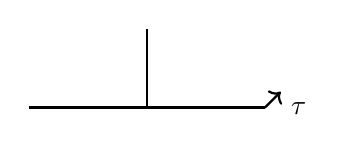
\begin{tikzpicture}
    \draw[thick] (0,0) -- (3,0);
    \draw[thick] (1.5,0) -- (1.5, 1);
    \draw[->, thick] (3,0) -- (3.2, 0.2) node[below right] {$\tau$};
\end{tikzpicture}
\end{center}

we'll have a completely flat retrospective (the correlation will be identical no matter the frequency we choose, since $R_h(\Delta_f) = \text{IFT}[S_h(\cdot)|\Delta_f] = \text{constant}$).
There are many technicalities, of course! In order to be able to write (3.77), we assume that the different resolvable delays are independent.

\begin{bluebox}[\faPen\ Uncorrelated Scattering (US) and WSSUS]
\begin{itemize}
    \item By \textit{resolvable delays} we mean delays $\tau_0 \neq \tau_1$ such that the channel's frequency response can be considered different between $\tau_0$ and $\tau_1$
    \item By independent, we imply that $\mathbb{E}[h(\tau_0)h^*(\tau_1)] = 0$ (which follows from their {\color{green!60!black} uncorrelation})
\end{itemize}
\end{bluebox}

The fact that $\mathbb{E}[h(\tau_0)h^*(\tau_1)] = 0$ for $\tau_0 \neq \tau_1$ is called the \textbf{uncorrelated scattering condition}, which, according to the book:

\begin{yellowbox}[\faBook\ \textit{Channel modeling} (pp. 131-208), p. 165]
is grounded in the reasonable premise that the propagation mechanisms giving rise to paths having resolvable delays are essentially independent. Together with the assumption of local stationarity, the uncorrelated scattering condition underpins the traditional modeling of small-scale fading \textbf{conforming the wide-sense stationary uncorrelated scattering (WSSUS) framework} introduced by Bello in 1963 [250]
\end{yellowbox}

Further note is that from (3.77) the uncorrelated scattering condition ensured that $R_h(\cdot)$ only depends on $\Delta_f$, not on $f$: this implies \textbf{the signal is wide sense stationary in the frequency domain as well}.

We then ask: when is a delay resolvable? We always use a pass band filter. If we're in baseband domain, we have a filter such as

\begin{center}
    \begin{tikzpicture}[>=Stealth, thick, line cap=round, line join=round, scale=1.5]
    % Main Horizontal axis line
    % Extending ends slightly past the features
    \draw (-2.5, 0) -- (3.5, 0);

    % Arrow tips at the far right
    % The main axis tip
    \draw[->] (3.4, 0) -- (3.6, 0);


    % Vertical axis line
    % Starts at the horizontal line and goes up (top is cut off in source image)
    \draw (0, 0) -- (0, 2.5);

    % The rectangle structure (centered on y-axis, sitting on x-axis)
    % Visually estimating proportions
    \draw (-1.2, 0) -- (-1.2, 1.3) -- (1.2, 1.3) -- (1.2, 0);

    % The arrow below indicating 'B'
    % Starts roughly under the center and points right
    \draw[->] (0, -0.8) -- (1.3, -0.8);

    % The label "B" below the arrow
    \node at (0.7, -1.3) {\Large B};

\end{tikzpicture}
\end{center}

which allows for perfect reconstruction if we sample at $T = 1/2B$.
What if we have another delay (meaning an actually wider bandwidth)? This means that a path will partly get its energy to neighboring paths:

\begin{center}
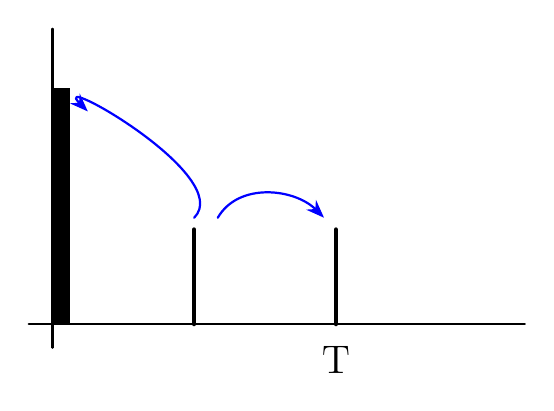
\begin{tikzpicture}[>=Stealth, thick, line cap=round, line join=round, scale=1.5]
    % Axes
    \draw[thick] (-0.2, 0) -- (4, 0); % x axis
    \draw[thick] (0, -0.2) -- (0, 2.5); % y axis

    % Pulse 1 (Main - Origin)
    % Depicted as a thick dark bar
    \fill[black] (0, 0) rectangle (0.15, 2.0);
    
    % Pulse 2 (at T)
    \draw[ultra thick] (1.2, 0) -- (1.2, 0.8);
    \node at (2.4, -0.3) {\Large T}; % Label T
    
    % Pulse 3 (at ~2T)
    \draw[ultra thick] (2.4, 0) -- (2.4, 0.8);
    
    % Blue Leaking Arrows
    % Arrow 1: From Main Pulse to Pulse 2
    % Curves from the side of the main pulse to the top of the second
    %\draw[->, blue, thick] (0.3, 1.5) to[out=45, in=135] (1.1, 0.9);

    \draw[->, blue, thick] (1.2, 0.9) to[out=45, in=135] (0.3, 1.8);
    
    % Arrow 2: From Pulse 2 to Pulse 3
    % Curves from the side/space of the second pulse to the top of the third
    \draw[->, blue, thick] (1.4, 0.9) to[out=60, in=135] (2.3, 0.9);

\end{tikzpicture}
\end{center}

This only works if the various paths are independent.
In the drawing up here they are dependent, since they come from the same real delay; if one goes down, the other will as well.

% Flowchart Highlight: Delay Spread
\begin{center}
\begin{tikzpicture}[
    node distance=1cm and 1cm,
    box/.style={
        rectangle, 
        draw=obsidianBorderPurple, 
        fill=obsidianPurple, 
        rounded corners, 
        align=center, 
        font=\footnotesize\sffamily,
        minimum height=1.5cm,
        inner sep=5pt
    },
    yellowbox/.style={
        rectangle,
        draw=yellow!80!orange,
        fill=obsidianYellow,
        align=center,
        font=\footnotesize\sffamily
    },
    arrow/.style={-Latex, draw=black!70}
]
    \node[yellowbox] (now) {Now};
    \node[box, below=0.1cm of now] (flatness) {Frequency flatness,\\ frequency correlation\\ and coherence\\ bandwidth};
    \node[box, right=of flatness] (relation) {Relation between\\ period, delays and\\ frequency-\\ flatness/selectivity};
    \node[box, right=of relation] (pdp) {Power delay profile\\ and its relation with\\ the frequency\\ correlation};
    
    % Highlighted box
    \node[yellowbox, below right=0.5cm and -0.5cm of pdp] (delay) {Delay spread in\\ continuous and\\ discrete cases};
    
    \node[box, above right=0.5cm and -0.5cm of pdp] (wssus) {WSSUS assumption};

    \draw[arrow] (flatness) -- (relation);
    \draw[arrow] (relation) -- (pdp);
    \draw[arrow] (pdp) -- (wssus);
    \draw[arrow] (pdp) -- (delay);
    \draw[arrow] (wssus) to[bend left=20] (pdp);
\end{tikzpicture}
\end{center}

Usually we have some parameters to describe the frequency fading; one is the \textbf{delay spread}

\begin{minipage}{0.6\textwidth}
\begin{equation}
    T_d = \sqrt{\int_{-\infty}^{+\infty} (\tau - \mu_\tau)^2 S_h(\tau) \, d\tau} , \tag{3.70}
\end{equation}
\end{minipage}
\begin{minipage}{0.35\textwidth}
\small
\textbf{Handwritten Note:}
\begin{align*}
    &\text{channel is flat} \\
    &\text{if } \quad B \ll B_c \\
    &\quad \quad \rotatebox{-90}{$\sim$} \quad \rotatebox{-90}{$\sim$} \\
    &\quad \quad \frac{1}{T} \quad \frac{1}{T_d}
\end{align*}
\end{minipage}

with $\mu_\tau$ being the average delay, expressed as
\begin{equation}
    \mu_\tau = \int_{-\infty}^{+\infty} \tau S_h(\tau) \, d\tau . \tag{3.69}
\end{equation}

$T_d$ is somewhat like measuring the variance, especially if we consider $S_h(\tau)$ as a PDF.
If the PDP happens to be discrete, than the delay spread is redefined as
\begin{equation}
    T_d = \sqrt{\sum_{q=0}^{Q-1} (\tau_q - \mu_\tau)^2 P_q} \tag{3.72}
\end{equation}
\[
\mu_\tau = \sum_{q=0}^{Q-1} \tau_q P_q ,
\]
which is nothing but an adaptation of (3.69), (3.70) with $S_h$ being a train of deltas weighted with $P_q$.

\begin{figure}[h]
    \centering
    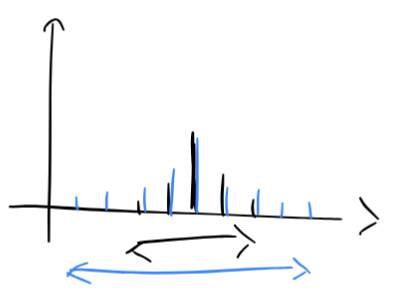
\includegraphics[width=0.5\textwidth]{Pictures/image copy 3.png}
\end{figure}

The blue channel is much more spread in time!
An ideal channel of course has just a path, thus RMS=0.
The smallest the RMS, the (generally) better. The principle of only having direct path is not something we like so much: by having only direct paths, sometimes the matrix might not be full rank anymore.

The channel is frequency flat if $T_d \ll T$. This means that \textbf{the symbol is much bigger than the delay, thus the ISI is so small that we can basically neglect it.}

This is like saying that the bandwidth $d$ is much less than the coherence bandwidth.
We thus have that the inequality in frequencies will be $B \ll B_c$:

\begin{figure}[h]
    \centering
    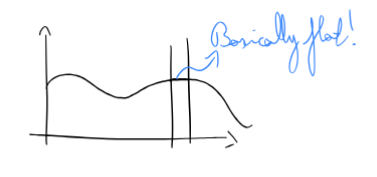
\includegraphics[width=0.6\textwidth]{Pictures/image copy 4.png}
\end{figure}

Oc it's really important to decide whether the channel is flat or not, as this allows to decide whether we need equalization or not.

\begin{tcolorbox}[colframe=red, colback=white, title=\faBolt\ Exam, fonttitle=\bfseries]
This would certainly be one question at the exam, if something needs to be asked about this chapter.
\end{tcolorbox}

The slides then state: "characterizing channels in terms of time, frequency and space coherence may be done under the unified framework of wide sense stationary uncorrelated scattering".
This is found under the acronym of \textbf{WSSUS}; this is the assumption we did until 15/20 years ago; nowadays the new channels can't have that being true anymore.
WSS means that $R_h$ only depends on $\Delta f$ (and not on $f$) or in other words that $S_h$ only depends on $\tau$ (and not on $t$).

When we use the WSSUS framework, everything becomes easier; we won't be requested to discriminate between the two, at least not in this course.

\subsection{Example 3.25: delay spread calculation}

Just as a reference, we have that the PDP is defined as

\begin{greenbar}
We can write down the \textbf{power delay profile (PDP)}, which \textbf{quantifies the energy distributed as a function of delay in the time domain}; it is normalized so that it can be interpreted as a PDF (describing how likely we are to have a certain amount of power at a certain delay) and it is denoted by
\begin{equation}
    S_h(\tau) = \mathbb{E}[|h(\tau)|^2]. \tag{3.68}
\end{equation}
\end{greenbar}

and its parameters instead are

If the PDP happens to be discrete, than the delay spread is redefined as
\begin{equation}
    T_d = \sqrt{\sum_{q=0}^{Q-1} (\tau_q - \mu_\tau)^2 P_q} \tag{3.72}
\end{equation}
\[
\mu_\tau = \sum_{q=0}^{Q-1} \tau_q P_q ,
\]
which is nothing but an adaptation of (3.69), (3.70) with $S_h$ being a train of deltas weighted with $P_q$.

The question of the example is "Compute the delay spread for the vehicular PDPs in Table 3.3"; table 3.3. is as follows:

\begin{center}
\captionof{table}{ITU vehicular PDP}
\begin{tabular}{cccc}
\toprule
\rowcolor{gray!50} \multicolumn{2}{c}{Vehicular A} & \multicolumn{2}{c}{Vehicular B} \\
\rowcolor{gray!20} Delay ($\mu$s) & Power share & Delay ($\mu$s) & Power share \\
\midrule
0    & 0.485 & 0    & 0.322 \\
0.31 & 0.385 & 0.3  & 0.574 \\
0.71 & 0.061 & 8.9  & 0.03 \\
1.09 & 0.048 & 12.9 & 0.057 \\
1.73 & 0.015 & 17.1 & 0.002 \\
2.51 & 0.005 & 20.0 & 0.014 \\
\bottomrule
\end{tabular}
\end{center}
\begin{purplebox}
\textbf{Handwritten Notes:}
\begin{itemize}
    \item ITU: International Telecommunication Union (United Agency of UN)
    \item IMT-2020 $\to$ 5G
\end{itemize}
\end{purplebox}

And describes the power share $S_h(\tau)$ for various delays in two setups, \textit{Vehicular A} and \textit{Vehicular B}.

By simply putting the numbers in the calculator, we'll find that $T_{d,A} = 0.37 \mu\text{s}, T_{d,B} = 4 \mu\text{s}$.

In vehicular channel, the \textbf{power share will eventually sum to 1} (so it can be considered just as if it was a probability distribution!).
The delays have very different values for the various channels. If we try to plot them, we can see that they are pretty different!

\begin{greybox}[\faCommentDots\ In-class blabbering]
When people are evaluating systems, they first of all establish the channel. The table shows an example for the ITU; 3GPP sends its standards to ITU; rn ITU is working on a standard called IMT-2030. Other organizations as well might be sending standards for evaluation at ITU, which have other channel models which might as well be different from the ones of 3GPP (3GPP might send 6G standard to ITU for evaluation).
5G has various techs, one of which is DECT-NR (NR: New Radio), which has been recognized by ITU as a 5G standard.

\textbf{We don't know which channel models reality the best}; when we select a certain technology, we want the tech to work well in both (or all) the channels we may be considering!
When it comes to models, there's a lot of uncertainty.

The power density profile is different; one goes down, the other goes up and down.
\end{greybox}

\newpage

\section{Single-user SISO}

\subsection{Introduction: capacity of AWGN channel, plotting $p_e$, various writings of $C$, total channel gain}

This chapter is revolving around the formula of capacity, trying to understand the relation between the various fundamental values.

We know we have that an AWGN channel has a capacity of
\[
C(\text{SNR}) = \log_2(1 + \text{SNR})
\]
achieved by using Gaussian distributed codewords.
In this chapter we'll see waterfilling and about the frequency selective channels.

We'll look at the capacity if the transmitter knows the channel information or if only receiver does or if both do.

We may be using \textbf{OFDM and not know the channel}: we'll use equal power for every carrier; of course if we use OFDM we at least need to know the lenght of the channel, as we'll need to set the cyclic prefix length accordingly. The energy we spend for the cyclic prefix is kind of wasted: we use it to simplify our relations, but it is wasted.
On top of that, if we know the channel we can distribute the power across the subcarriers in an optimum way. This is why we use \textbf{pilots}: using them, we can estimate the channel. This as well can be seen as a \textit{waste}, since we could be transmitting information; point is that then the receiver gets to know the channel; if the receiver feeds the info of the channel back to the transmitter, then the transmitter can optimize itself.

From the last chapter we know the RMS of the channel; we generally interpret that to be Gaussian. We can then make some assumptions and verify if they're true (starting with equal power) and then we'll have a \textbf{return channel} used to gather feedback from the receiver.
This feedback loop is crucial if we want to get the most out of OFDM. Another thing is that the feedback channel is such that we send some information related to the channel itself.
It's also important to take into account the fact that we'll need to quantize our channel: how many bits should we use to quantize the channel? This is an open problem!

\begin{greenbar}
There are many papers discussing this; the amount of bits used are really variable.
\end{greenbar}

Usually we have an idea, we implement and measure the performance: the difference is called \textbf{implementation gap}. We'll be left with a high probability of error, which will be in dB.
The simple idea used in practical system in order to measure the error in dB is to have a curve such as:

\begin{center}
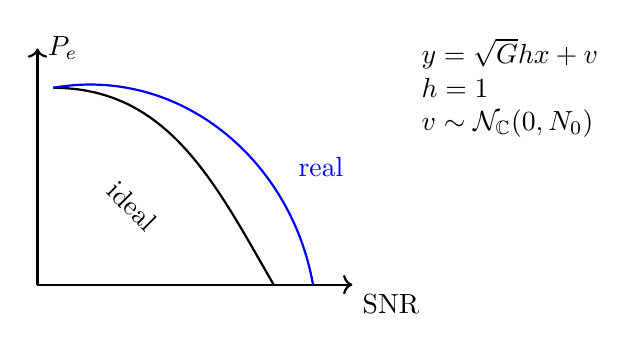
\begin{tikzpicture}
    % Axis
    \draw[thick, ->] (0,0) -- (4,0) node[below right] {SNR};
    \draw[thick, ->] (0,0) -- (0,3) node[right] {$P_e$};
    
    % Curves
    \draw[thick] (0.2, 2.5) to[out=0, in=120] (3, 0);
    \node at (1.2, 1) [rotate=-45] {ideal};
    
    \draw[thick, blue] (0.2, 2.5) to[out=10, in=100] (3.5, 0);
    \node[blue] at (3.6, 1.5) {real};
    
    % Equations top right
    \node[align=left] at (6, 2.5) {$y = \sqrt{G}hx + v$ \\ $h=1$ \\ $v \sim \mathcal{N}_{\mathbb{C}}(0, N_0)$};
\end{tikzpicture}
\end{center}
We select a certain value and then we measure a distance, which is in dB:

\begin{center}
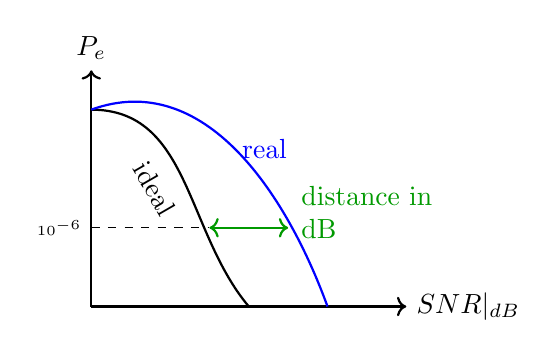
\begin{tikzpicture}
    % Axis
    \draw[thick, ->] (0,0) -- (4,0) node[right] {$SNR|_{dB}$};
    \draw[thick, ->] (0,0) -- (0,3) node[above] {$P_e$};
    
    % Curves
    \draw[thick] (0, 2.5) to[out=0, in=130] (2, 0);
    \node at (0.8, 1.5) [rotate=-60] {ideal};
    
    \draw[thick, blue] (0, 2.5) to[out=20, in=110] (3, 0);
    \node[blue] at (2.2, 2) {real};
    
    % Distance measurement
    \draw[<->, green!60!black, thick] (1.5, 1) -- (2.5, 1);
    \node[green!60!black, align=left] at (3.5, 1.2) {distance in\\dB};
    
    % Label 10^-6 approx location
    \draw[dashed] (0, 1) -- (1.5, 1);
    \node[left] at (0, 1) {\tiny $10^{-6}$};
\end{tikzpicture}
\end{center}

And then how do we implement the return channel?

\begin{center}
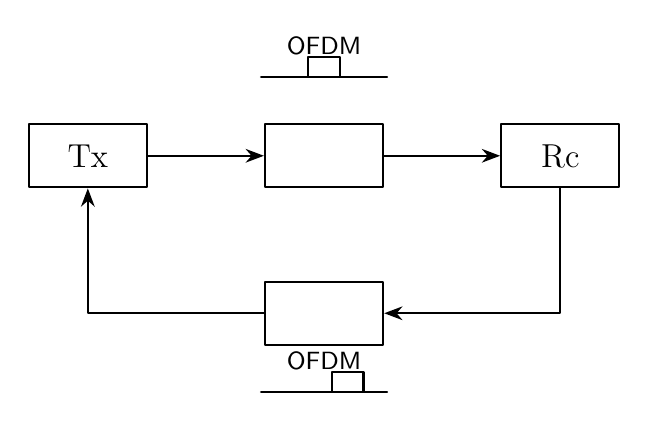
\begin{tikzpicture}[>=Stealth, thick, line cap=round, line join=round, scale=1]

    % Stile dei blocchi
    \tikzset{block/.style={draw, rectangle, minimum width=1.5cm, minimum height=0.8cm, align=center}}

    % Nodi principali (Tx, Canale diretto, Rx, Canale di ritorno)
    \node[block] (tx) at (0, 0) {\large Tx};
    \node[block] (ch) at (3, 0) {}; % Box vuoto centrale superiore
    \node[block] (rx) at (6, 0) {\large Rc}; % "Rc" come da disegno
    
    \node[block] (fb) at (3, -2) {}; % Box vuoto centrale inferiore (feedback)

    % Frecce percorso diretto
    \draw[->] (tx) -- (ch);
    \draw[->] (ch) -- (rx);
    
    % Frecce percorso di feedback
    % Dal ricevitore al blocco di feedback (esce da sotto, entra da destra)
    \draw[->] (rx.south) |- (fb.east);
    
    % Dal blocco di feedback al trasmettitore (esce da sinistra, entra da sotto)
    \draw[->] (fb.west) -| (tx.south);

    % --- Elemento OFDM Superiore ---
    \begin{scope}[yshift=1cm, xshift=3cm]
        \node at (0, 0.4) {\sffamily\small OFDM}; % Testo
        \draw (-0.8, 0) -- (0.8, 0);       % Linea base
        \draw (-0.2, 0) rectangle (0.2, 0.25); % Impulso rettangolare
    \end{scope}

    % --- Elemento OFDM Inferiore ---
    \begin{scope}[yshift=-3cm, xshift=3cm]
        \node at (0, 0.4) {\sffamily\small OFDM}; % Testo
        \draw (-0.8, 0) -- (0.8, 0);       % Linea base
        \draw (0.1, 0) rectangle (0.5, 0.25);  % Impulso (leggermente spostato come nel disegno)
    \end{scope}

\end{tikzpicture}
\end{center}

We can't assume that the return channel is error-free, of course.

We need to have a reliable link; having probability of error equal to 0 means we'd need to have a code with a block length which is very large (actually, infinite). Point is that such a code would give a pretty large delay, while our problem is also that we'd like to have a small delay: if we have too much, by the time we deliver info about the channel, it has already changed.

Normally in the books this is forgotten, but it's important: we need to change this so that we're bringing \textbf{not-too-much service information around}; if we don't, we're not bringing any user information.

\begin{center}
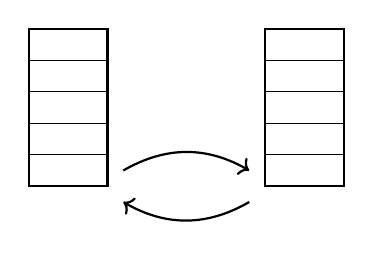
\begin{tikzpicture}
    % Stack 1
    \draw[thick] (0,0) -- (0,2) -- (1,2) -- (1,0) -- cycle;
    \foreach \y in {0.4, 0.8, 1.2, 1.6} \draw (0,\y) -- (1,\y);
    
    % Stack 2
    \draw[thick] (3,0) -- (3,2) -- (4,2) -- (4,0) -- cycle;
    \foreach \y in {0.4, 0.8, 1.2, 1.6} \draw (3,\y) -- (4,\y);
    
    % Arrows
    \draw[->, thick, bend left] (1.2, 0.2) to (2.8, 0.2);
    \draw[->, thick, bend left] (2.8, -0.2) to (1.2, -0.2);
\end{tikzpicture}
\end{center}

We're mostly interested about the exchange of billing information.

We could see \textbf{many formulations of the formula of capacity}; we can find
\begin{equation}
    C = \frac{1}{2}\log_2(1 + \text{SNR}) \quad [\text{bits/use} \leftrightarrow \text{bits/s/Hz}] ;
\end{equation}
the $\frac{1}{2}$ depends on whether we're considering the channel as complex (no $1/2$) or not (has $1/2$). We have no $B$ in front of the equation before; without $B$ is the capacity per channel use; we suppose we use the channel with an interval $T=1/B$, meaning that the rate at which we use the channel is $B$.

This is why we might also find
\begin{equation}
    C = B \log_2(1 + \text{SNR}) \quad [\text{bits/s}] .
\end{equation}

Let's then consider
\[
\log_2(1 + \text{SNR}) :
\]
which is the range for SNR? Normally it is $\in [0, \infty)$.
We might as well express it as dB: the SNR can get really close to 0, meaning that for $\text{SNR} = 0$, we get a capacity of 0.

We of course have
\[
\text{SNR}|_{dB} = 10 \log_{10} \text{SNR} .
\]

Of course if in dB we can have a negative value, meaning that the signal has less power than the noise.

We need to measure the SNR at the point of decision; there are systems working at \textbf{negative SNR in dB}, meaning that the power of the noise is much higher than the power of the signal; what is the use case? Military use! In the army we don't want the enemy to get the message, even if it is encrypted; if my transmission is detected, the radar can detect where I am (we just have 2 receivers which can understand the location by looking at the power while they rotate). We don't even want the enemy to know we're transmitting. If we stay below a certain transmission noise, we can accomplish this!
LORA is such that if we transmit very far, the power goes below the level of the noise.
If we've seen a different kind of modulation, we see that we can also work on the other side; the way to do this is to use DSSS ({\color{green!60!black} \underline{Direct Sequence Spread Spectrum}}): we have a +1, -1 signal and we multiply this with a pseudo-random sequence

\begin{figure}[h]
    \centering
    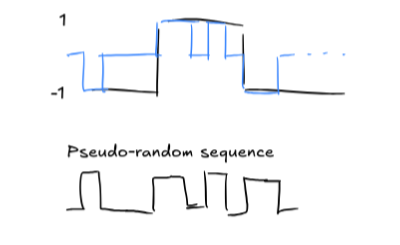
\includegraphics[width=0.5\textwidth]{Pictures/image copy 5.png}
\end{figure}

We're spreading this signal to a larger spectrum, eventually going below the level of noise. How do I recover the signal? I multiply again by the +1, -1 we had before, getting back the original signal. We get back to a small bandwidth: we have again sufficient SNR for reliable transmission.

\begin{greenbox}
This is just a silly PAM, but we could apply it to more elaborate trasmissions.
\end{greenbox}

\begin{figure}[h]
    \centering
    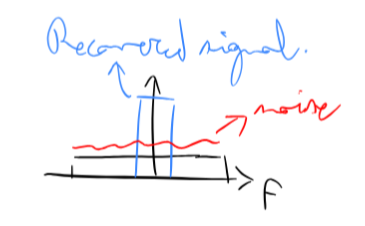
\includegraphics[width=0.5\textwidth]{Pictures/image copy 6.png}
\end{figure}

We know the SNR at which a certain model/protocol will work!
We look at the SNR at the point in which we'll transmit; we don't care about what happens in the rest of the channel.

\begin{greenbox}
The crucial point for this lecture was understanding whether we could put the $\frac{1}{2}$ or $B$ in the equations.
\end{greenbox}

The key SISO quantities are the \textbf{bitrate, transmit power and bandwidth}, $R, P_t, B$. Normally the bandwidth is given; sometimes, we can decide to enlarge the bandwidth, switch it etc etc; now GPS is not reliable because when it was conceived, the bandwidth was large enough that it was impossible to jam the signal in there. Now it's actually really easy.
We know the frequency at which GPS is transmitting and we can make the receiver/transmitter blind.

The rate here would be referenced to the channel capacity; this means that we always compare the rate ($R$) to the channel capacity; we need to know if we're far from the channel capacity or if we're close to it. If we're far, we need to work.


Of course the channel capacity and the channel gain play a central role in the formulation of the tradeoffs between $R, P_t$ and $B$. The \textbf{total channel gain} is, by definition, the ratio between the received and the transmit signal powers, aka
\begin{equation}
    \frac{\mathbb{E}[|\sqrt{G}hx|^2]}{\mathbb{E}[|x|^2]} = G \frac{\mathbb{E}[|hx|^2]}{E_s} , \tag{4.1}
\end{equation}
which will normally consist in attenuation; we'll only have gain if we include antennas.
When we want to calculate $\mathbb{E}[|hx|^2]$, is it safe to say it is $= \mathbb{E}[|h|^2]\mathbb{E}[|x|^2] = 1 \cdot E_s$? \textbf{Only if they're uncorrelated!} This happens for fading-independent transmissions, in which $x$ is independent of the unit-power small-scale channel coefficient $h$.
If the signal and channel are uncorrelated, then we have that the total channel gain is equal to $G$.

\begin{yellowbox}[\faBook\ \textit{Single-user\_SISO} (pp. 209-294), p. 2]
To illustrate the various definitions and relationships put forth in this section, we have the running example of the channel $y = \sqrt{G}hx + v$ with $h=1$ and $v \sim \mathcal{N}_{\mathbb{C}}(0, N_0)$. This basic channel, which permeates many of the derivations in Chapter 1, is termed the AWGN channel because it is only impaired by AWGN; its capacity function, borrowed here and then formally derived in Section 4.3, is $C(\text{SNR}) = \log_2(1 + \text{SNR})$.
Delving into the tradeoffs between $R, P_t$, and $B$, we begin by observing that, rather than relate these quantities directly, it is preferable to relate the ratios $R/B, P_t/B$, and $P_t/R$, which happen to have an operational importance of their own.
\end{yellowbox}

\begin{tcolorbox}[colframe=red, colback=white, title=\faBolt\ Exam, fonttitle=\bfseries]
We should have in mind the order of magnitude of $N_0$. Let's say at the exam professor says like $N_0 = ???$; what's the order of magnitude of that? In the book we find it is $10^{-20} \text{W}/\sqrt{\text{Hz}}$.
\end{tcolorbox}

\section{POTS and telephone system detour}

POTS (telephone system; we then had ISDN (Integrated System Digital Network); nowadays we only have the IP network); even in the IP network we have control traffic: we need to exchange info about the routing tables.

\begin{bluebox}[\faPen\ About fixed phones]
An example: we pick up the phone; we hear the tone, which means that the line is available. Some time ago, it could happen to not hear the tone of three line, but the busy line tone. We're using a protocol in this exchange of information. Once we get the line, we start making the number; the network will understand when we're finished writing. Then there's a dialogue between various nodes to understand where the person we're calling is.
If the other person is found, their phone starts ringing. Only when the other person picks up, the user data starts. Once the phone is put on hook, there's another signal saying \textit{the communication has been closed}.
Mobile phones use a different protocols: they don't know when we've finished putting the number. This is why we have the green number.

\begin{greenbar}
At the time we had a phone sending impulses to the local switch; when the phone which turned sent an impulse at every tick while coming back. If we pressed 9, for example, there was just 1 tick.
The one with the buttons understood the numbers in another way; it still was connected to the central exchange; info was covered using the DTMF (Dual Tone MultiFrequency); we have various different frequencies: depending on what we press, we'll get a different transmitted signal. The tones (=frequencies) are such to give the coordinates of the number that we want to call.
The prefix code is what's used for the communication, actually. If we have a double 0 at the start, the network understands we want to go outside of italy; by pressing \texttt{00} we express the fact that we want to go somewhere else. We then have country codes: \texttt{3,4} mean \textit{europe}. Italy is \texttt{039}: of course we can't have a country with a prefix of \texttt{0391}, because otherwise italy wouldn't be valid anymore.
If we have \texttt{039049} this means we want to contact Padova.
There must be a worldwide agreement on the numbers. The CEPT is the one assignining the prefixes.
\end{greenbar}
\end{bluebox}

That of the phone was the \textbf{first example of standardization}; we cannot do this with the mobile phone since mobile phones are digital; it would be a nightmare to find codes related to mobile networks: they are ISDN numbers. In the mobile network there's another \textit{hidden} number which allows us to (for example) change operator.
If we send a message, sending a number one by one would definitely congest the network. It was preferred to have the green button and send the message all at once.

\begin{greenbar}
Random story on the africa linking between the satellitar and \textit{terrestrial} network; terrible fiasco rip.
\end{greenbar}

We need to have a function which should inform the network about the location of a certain phone; if an italian phone is in egypt, network contacts the number; HRR is contacted and that register knows where you are.
We can then transfer our request to connect to the register network.
The operator does not know where we are exactly, as this would be too much information to hold; the cell is too much informaiton as well; they did a location area, which is a set of cells such that if our cell is in there and not engaged in a call: how many cells there are depends on our network design; the location area is written in the HRR: when a call reaches us, the cell broadcasts information: it tells which people are requested to connect every certain amount of milliseconds; the phone understands that message and if it is requested to connect to a call, it starts the transmission. The resource is so scarse that we only allocate it when we know that the transmission is going well.

\begin{greenbar}
The network keeps track of what's happening in order to send the bill; we then need to read the bills and understand if the person was at a certain location or not.
\end{greenbar}

\section{Infineon detour}

Infineon detour; he talked about what infineon does and what they sell to who.

Aurix: architecture designed for cars; this is needed since the interrupts need to be served really quickly. Their processors range in various power values. The ones who made Aurix are mostly focused in analog, they develop the peripherals for the car.
They are developing telecom systems: one example is the mandatory system which detects how many people are in the car when we close it. More than that, we also need to sense the environment and whether the driver is fully awake.
Another example are the sensors which detect whether we're drunk.

Infineon is a very good place to work: they take care of people for their growth; salaries are aligned with the international market; open positions are first broadcast to internal people. We then have a lot of project management: when working in automotive it's needed to design things really carefully.


They also need to comply with many regulations.
Infineon uses machine learning in order to ensure a really good production yield (e.g.: they use ML to have a frequency as close as possible to the desired one).

\begin{greenbar}
We can also decide whether we want to continue with a technical career or a managerial career.
\end{greenbar}

\begin{tcolorbox}[colframe=red, colback=white, title=\faBolt\ What is the structure of the exam?, fonttitle=\bfseries]
First of all, we might be checked on the background.
The first part is closed book. We can have 1A4 paper which must have our name and student id; we can only write on the front!!
At the start of the exam, all our cheat sheets will be put on the desk and we won't be able to look at them. We'll then need to answer to ten questions in a \textit{crocette} format. We then have a theoretical exercise: example "prove that the MMSE estimator is ...": there are no numbers here! The first exercise is a theoretical exercise. We'll have 2 sets of papers; when we decide we have finished, we can deposit the theoretical part and pick up the cheat sheet: we'll then have a numerical exercise, in which there \textit{will} be numbers.
We of course need to put together our sequence number.
We can also take a calculator with us, but it shall not be connected to the internet.
\end{tcolorbox}

\begin{greenbar}
For tomorrow's tutor lecture, professor selected some exercises.
\end{greenbar}

\section[SNR and several other definitions]{SNR (+several other definitions: spectral efficiency, transmit energy, energy per bit); expressions of capacity $C, \mathbb{C}$}

We know that the \textbf{spectral efficiency} is how many bits we can send per Hz: it's $R/B$; the unit is
\[
\frac{\text{b/s}}{\text{Hz}} :
\]
If I have a spectral efficiency of 100 [b/s/Hz] and we have 4 Hz, we can send 400 [bit/s]: if we enlarge our $B$, we're improving the channel; of course we can't do this without any limit: we know that the capacity is an upper bound to the amount of bps we can send. If we know the receive power, the number of bits per hertz has a limit which is the Shannon bound.

We have as a rule of thumb that we transmit with period $T = 1/B$; what actually happens is that we use a little bit more than $B$, as we know (since we can't really use $rect$ signals in frequency, as they'd give an endless signal in time).

The \textbf{transmit energy} is
\begin{equation}
    P_t/B = P_t T = E_s = \mathbb{E}[|x|^2] .
\end{equation}
The SNR must be measured \textbf{at the decision point}; we see that
\begin{align}
    \text{SNR} &= \frac{GP_t/B}{N_0} \tag{4.2} \\
    &= \frac{GE_s}{N_0} : \tag{4.3}
\end{align}
this is measured at the receiver, at the decision point (this means that we're doing this at the receiver). Why is $B$ there? It can be put below, as $BN_0$ is the power of the noise.

Instead, $P_t/R$ is the \textbf{energy spent per bit} (this is because $R$ is in bits/s); this is at the receiver (we can tell this as we have $G$):
\begin{align}
    E_b &= G \frac{P_t}{R} \tag{4.4} \\
    &= \frac{GE_s}{R/B} : \tag{4.5}
\end{align}
this is an especially useful quantity when referred to $N_0$ (we'll see it's often used as a reference values for our graphs); specifically, it gives
\begin{align}
    \frac{E_b}{N_0} &= \frac{1}{N_0} \frac{GE_s}{R/B} \tag{4.6} \\
    &= \frac{\text{SNR}}{R/B} . \tag{4.7}
\end{align}

\begin{greenbar}
This is just a game of substitution.
\end{greenbar}

$E_b$ is the energy per bit; the value $E_b/N_0$ is generally put on the $x$ axis: we can see (as it is clear from (4.7)) that it is linked to the SNR.

\begin{greenbar}
Sometimes it's not so obvious where the \textit{decision point} is.
\end{greenbar}

We've already seen the capacity bounds; $C$ is the capacity we have seen quite some time ago; we also have the power $P_t$, though. They give:
\begin{align}
    R &= B \cdot C \left( \frac{GP_t}{N_0 B} \right) = B \cdot C(\text{SNR}) \tag{4.12} \\
    P_t &= \frac{N_0 B}{G} C^{-1} \left( \frac{R}{B} \right) . \quad \xrightarrow{\text{\tiny how much power to transmit to get at the capacity}} \tag{4.13}
\end{align}

Depending on the reference framework we choose to adopt, we can move across one another following the scheme below:

\begin{figure}[h]
    \centering
    
\includegraphics[width=0.8\textwidth]{Pictures/immagine-002.png}
\end{figure}

Problem here is in the notation: we have two different notations of capacity, $\mathsf{C} \neq C$.

We have that
\[
C(\text{SNR}) = \log(1 + \text{SNR})
\]
but we can also write this using
\[
\text{SNR} = \frac{B}{R} \frac{E_b}{N_0}
\]
giving
\[
\log \left( 1 + \frac{B}{R} \frac{E_b}{N_0} \right) ,
\]
which is a different function from $C(\text{SNR})$: we have $\boxed{\mathsf{C}\left(\frac{E_b}{N_0}\right)}$. We might want to plot the capacity as a function of either the SNR or as a function of $E_b/N_0$.
From the triangle we see that on the left we have $C$ and on the right we have $\mathsf{C}$.

\begin{tcolorbox}[colframe=red, colback=white, title=\faBolt\ Exam, fonttitle=\bfseries]
In the exam, normally $C$ is reserved for the capacity formula: we need to make it clear what the formula we're using is.
\end{tcolorbox}

From the fact that $C = \mathsf{C} = R/B$, we can write that
\begin{equation}
    \frac{E_b}{N_0} = \frac{\text{SNR}}{C(\text{SNR})} \tag{4.8}
\end{equation}
and
\begin{equation}
    \text{SNR} = \frac{E_b}{N_0} \mathsf{C} \left( \frac{E_b}{N_0} \right) . \tag{4.9}
\end{equation}

The reason why the link between $P_t, B$ has \textit{no function} is that in those situations we don't know what $R$ is, thus it's not easy to go from one to the other. \scriptsize \textit{Per i figli, fino a 4.3} \normalsize

\end{document}

